\documentclass[a4paper, 12pt]{article}
\renewcommand{\baselinestretch}{1.5}
\usepackage{algorithm}
\usepackage{arevmath}     % For math symbols
\usepackage{algpseudocode}
\usepackage{mathtools}
\usepackage{fontspec}
\usepackage{graphicx}
\usepackage{tabularx}
\usepackage{setspace}
\usepackage{longtable}
\usepackage{amsmath}
\usepackage{unicode-math}
\usepackage{capt-of}
\usepackage{sectsty}
\usepackage{stackengine}
\usepackage{hyperref}
\usepackage{caption}
\usepackage{titlesec}
\usepackage{subcaption}
\usepackage{array,ragged2e}
\usepackage[justification=centering]{caption}
\usepackage[format=hang,font={small,bf},labelfont=bf]{caption}
\usepackage{nomencl}
\usepackage{siunitx}
\usepackage{etoolbox}
\makenomenclature
\usepackage[sorting=none]{biblatex} %Imports biblatex package
\addbibresource{ref.bib} %Import the bibliography file
\defbibheading{References}[\bibname]{%
  \section*{\centering #1}%
  \markboth{#1}{#1}}
\newcommand\xrowht[2][0]{\addstackgap[.5\dimexpr#2\relax]{\vphantom{#1}}}
\usepackage[margin=1in]{geometry}
\usepackage{tocloft}
\hypersetup{draft}
%  \pagestyle{empty}
\setmainfont{Times New Roman}
\captionsetup[figure]{font={small, bf},labelfont={bf},name={Fig.},labelsep=period}
\renewcommand{\algorithmicrequire}{\textbf{Input:}}
\renewcommand{\algorithmicensure}{\textbf{Output:}}
\renewcommand{\nomname}{\makebox[\linewidth]{Nomenclature}}%
\renewcommand{\contentsname}{\hfill\bfseries\Large Contents\hfill}
\renewcommand{\cftaftertoctitle}{\hfill}
\sectionfont{\fontsize{18}{18}\selectfont}
\setcounter{tocdepth}{4}
\setcounter{secnumdepth}{4}
\titleformat{\paragraph}
{\normalfont\normalsize\bfseries}{\theparagraph}{1em}{}
\titlespacing*{\paragraph}
{0pt}{3.25ex plus 1ex minus .2ex}{1.5ex plus .2ex}

\begin{document}
\pagenumbering{roman}
\setcounter{page}{1}
\tableofcontents
\newpage
\begin{center}
\phantomsection
\listoftables
\addcontentsline{toc}{section}{\listtablename}
\end{center}
\newpage
\begin{center}
\phantomsection
\listoffigures
\addcontentsline{toc}{section}{\listfigurename}
\end{center}
%% This code creates the groups
% -----------------------------------------

\renewcommand\nomgroup[1]{%
  \item[\bfseries
  \ifstrequal{#1}{E}{Non-English Alphabets}{%
  \ifstrequal{#1}{C}{English Alphabets}{%
  \ifstrequal{#1}{I}{Abbreviations}{%
  \ifstrequal{#1}{O}{Other symbols}{}}}}%
]}
% -----------------------------------------
%% This will add the units
%----------------------------------------------
\newcommand{\nomunit}[1]{%
\renewcommand{\nomentryend}{\hspace*{\fill}#1}}
%----------------------------------------------
\newpage
\phantomsection{}
\printnomenclature
\nomenclature[E]{\(\alpha\)}{Alpha}
\nomenclature[E]{\(\beta\)}{Beta}
\nomenclature[E]{\(\epsilon\)}{Epsilon}
\nomenclature[E]{\(\sigma\)}{Sigma}
\nomenclature[E]{\(\sum\)}{Uppercase Sigma}
\nomenclature[E]{\(\omega\)}{Omega}

\nomenclature[C]{\(e\)}{Euler's constant \nomunit{\(2.71828\)}}



\nomenclature[I]{\(ANN\)}{Artificial Neural Network}
\nomenclature[I]{\(ARCH\)}{Autoregressive Conditional Heteroscedasticity}
\nomenclature[I]{\(AUC\)}{Area Under Curve}

\nomenclature[I]{\(BN\)}{Bayesian Network}
\nomenclature[I]{\(CART\)}{Classification and Regression Trees}
\nomenclature[I]{\(DAG\)}{Directed Acyclic Graph}
\nomenclature[I]{\(DT\)}{Decision Tree}
\nomenclature[I]{\(EDA\)}{Exploratory Data Analysis}
\nomenclature[I]{\(GARCH\)}{Generalized Autoregressive Conditional Heteroskedasticity}
\nomenclature[I]{\(KNN\)}{K-Nearest Neighbours}
\nomenclature[I]{\(LCR\)}{Liquidity Coverage Ratio}
\nomenclature[I]{\(LR\)}{Logistic Regression}
\nomenclature[I]{\(LDA\)}{Linear Discriminant Analysis}
\nomenclature[I]{\(MLP\)}{Multilayer Perceptron}
\nomenclature[I]{\(MSE\)}{Mean Squared Error}
\nomenclature[I]{\(NSFR\)}{Net Stable Funding Ratio}
\nomenclature[I]{\(NPA\)}{Non Performing Assets}
\nomenclature[I]{\(RBI\)}{The Reserve Bank of India}
\nomenclature[I]{\(RF\)}{Random Forest}
\nomenclature[I]{\(ROC\)}{Receiver Operating Characteristics}
\nomenclature[I]{\(SVM\)}{Support Vector Machine}
\nomenclature[I]{\(VAR\)}{Value at Risk}
\addcontentsline{toc}{section}{Nomenclature}
\newpage
\begin{center}
\phantomsection
\section*{\centering Abstract}
\addcontentsline{toc}{section}{Abstract}
\end{center}
\textit{
{\fontsize{10pt}{10pt}\selectfont Banking forms the backbone of modern society. With banks serving millions of customers from every corner of the world, it becomes crucial for banks to stay competitive, sustainable and at the same time work under compliance constraints. Risk management is an area of study which aims to reduce fraud, improve processes and decrease losses to the banking industry. Several state-of-the-art machine learning and statistical models are used to identify, analyze and mitigate risks for the organizations. These models are exceedingly improved by the terabytes of data that banks generate daily. This report presents a comprehensive analysis of various techniques used for risk management in the banking sector. A comparative study is performed on various machine learning models and their strengths for different risk management tasks. Finally, a case study is also presented highlighting the complete process of a sample risk management task for credit scoring.
}
}
\vskip 0.1in
\noindent\
\emph{
{\fontsize{10pt}{10pt}\selectfont \textbf{Keywords:}  Banking - Risk Management - Machine Learning - Credit Score}}

\begin{center}
\newpage
\pagenumbering{arabic}
\setcounter{page}{1}
\section{\centering Introduction}
\end{center}
\vskip 0.25in
The banking industry is an essential part of the global economy handling over 150 trillion U.S Dollars worth of global assets. Amidst the economic recession caused due to the COVID-19 pandemic, the total value of banking-related fraud in India doubled from Rs 71,534 Crores in 2018-19 to Rs 1,38,422 Crores in the fiscal year  2020-21 \cite{rbi21}. Global recessions like the 2008 Financial Crisis and the recent COVID-19 pandemic slows down economic output and put a lot of pressure on financial institutions, especially banks. Having a strong infrastructure to manage and mitigate financial risk becomes crucial to keeping the global economic engine running.
\vskip 0.2in
\noindent
Over the last few decades, advancements in Machine Learning have been extensively utilized to help in risk management tasks. With almost all financial instruments running in a digital form, machine learning models are employed extensively to detect fraud, predict commodity prices, track inflation etc. A lot of research has been done academically and in the industry since the 2008 Financial Crisis to build state of the art models for various risk management activities. This report presents a summary of multiple machine learning techniques that are used to solve a variety of risk management related problems.
\vskip 0.2in
\subsection{Applications}
Risk management is a 17.1 Billion U.S. Dollar industry responsible for handling inflation, financial frauds, cyber threats, market volatility etc. \cite{bcc17}. Machine Learning models significantly improve the accuracy of existing risk management tasks and can do so globally by working on petabytes of data that the banking sector produces daily. Typical applications of machine learning in risk management tasks include:

\begin{itemize}
  \item \textbf{Credit Risk:} Determining if the borrower can repay the loan.
  \item \textbf{Market Risk:} Predicting volatility and movement in commodity and equity markets.
  \item \textbf{Financial Fraud Risk:} Identifying money laundering patterns from transactions.
  \item \textbf{Liquidity Risk:} Identifying stability of sectors before investing in financial instruments
  \item \textbf{Operational Risk:} Detecting Fraud and suspicious transactions
\end{itemize}






\vskip 0.2in
\subsection{Motivation}
Risk Management is essential for a country's economy. The Reserve Bank of India (RBI) reported the presence of about Rs. 900 Thousand Crores of Non-Performing Assets (NPA) in 2020 in the Indian banking sector \cite{rbi20}. These are essentially bank loans that are in default or arrears. This amount of loss is roughly equivalent to the cost to build an international airport in India. Machine Learning plays a monumental role in reducing exposure to such risks, which can significantly impact national and global economies.
\vskip 0.2in
\subsection{Objectives}
This report aims to summarize the work done in risk management in the banking sector from a machine learning point of view. Additionally, this report also presents a case study comparing the performance of different machine learning models to evaluate credit risk on a single dataset.
\vskip 0.2in
\subsection{Organization of Report}
This report is subdivided into five chapters. The first chapter gives an overview of the banking industry along with the applications, motivations and objectives of this report. The second chapter provides the necessary theoretical background on machine learning algorithms and concepts related to banking and risk management. The third chapter presents a comparative study of various academic work done for different risk management tasks using machine learning. The fourth chapter is a case study for a particular risk management problem that builds upon the previous chapters and reports the results of various machine learning algorithms. The final chapter concludes all the findings of the seminar report in a concise format.
\newpage

\section{\centering{Theoretical Background}}
\vskip 0.25in
This chapter is subdivided into two parts. The first part is a brief outline of standard machine learning models and terminologies. The second part explains various terminologies related to finance, banking and risk management.
\vskip 0.2in
\subsection{Machine Learning Algorithms}
\subsubsection{Logistic Regression (LR)}
\begin{center}
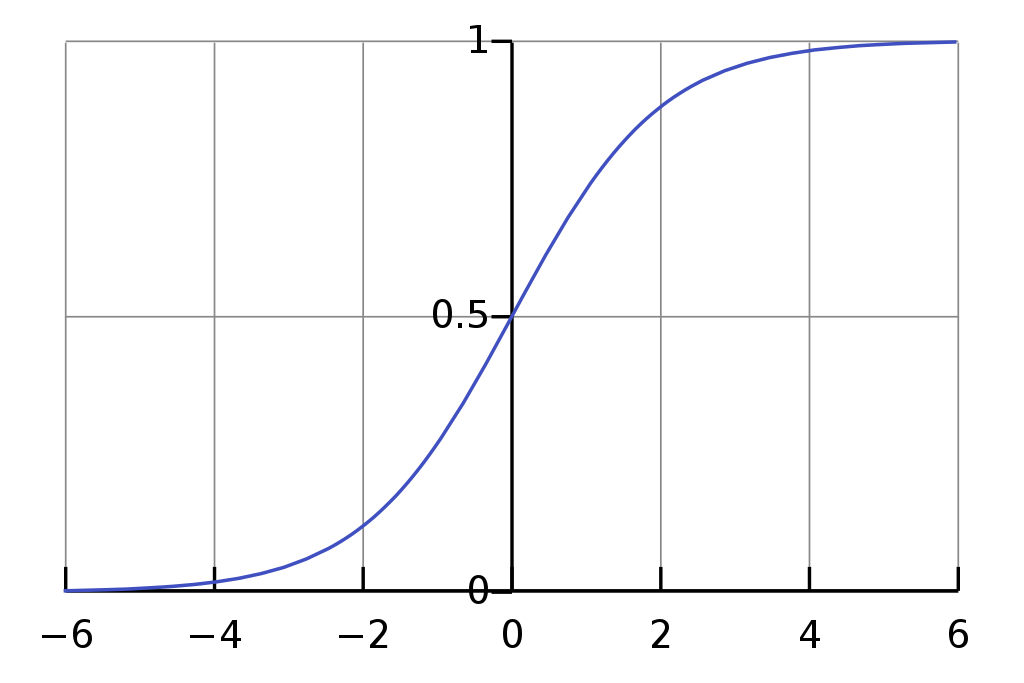
\includegraphics[scale=0.3]{lr.png}
\captionof{figure}{Logistic function curve}
\label{fig:lr}
\end{center}
In statistics, LR models the probability of a specific class or event happening. This probability estimate is further used for binary classification and with minor extensions to perform multi-class classification. The algorithm is based on a logistic function which is a sigmoidal curve. It takes a real-valued input and outputs a number between zero and unity (Fig. \ref{fig:lr}). This output is interpreted as the probability of the task. Mathematically, the logistic function is represented as follows:
\begin{equation}
\sigma(t) = \frac{e^t}{1 + e^t} = \frac{1}{1 + e^{-t}}
\end{equation}
If \(t\) is derived from a single independent linearly varying variable \(x\), the generalized logistic function can be represented as follows:
\begin{equation}
    t = \beta_0 + \beta_1x
    \end{equation}
    \begin{equation}
    p(x) = \sigma(t) = \frac{1}{1 + e^{\beta_0 + \beta_1x}}
\end{equation}
\vskip 0.2in
\subsubsection{Decision Tree (DT)}
\noindent Decision Tree Learning involves the construction of DTs, which will be traversed to conclude a given set of observations of data points. Classification Trees are models where the predicted outcome is discrete. Decision Tree training algorithms work in a top-down fashion to split the data set at every stage using a specific metric. Popular decision trees and their splitting metrics are discussed below.
\vskip 0.2in
\noindent\textbf{Classification and Regression Tree (CART)} \\
\noindent CART model uses the Gini Impurity Index \(I_G\) as its splitting parameter, which is computed for \(j\) classes as follows:
\begin{equation}
    I_{G}(p) = 1 - \sum_{i = 1}^{j} p_i^2
\end{equation}
\vskip 0.2in
\noindent\textbf{Information Gain based DTs} \\
\noindent DT models like ID3, C4.5 and C5.0 use information gain, which is based on the entropy  of the dataset. Mathematically Entropy \(H\) and Information Gain \(IG\) for \(j\) classes are defined as below:

\begin{equation}
    H(T) = - \sum_{i=1}^{j} p_i \log_2 p_i
\end{equation}

\begin{equation}
    IG(T, a) =  H(T) - H(T|a)
\end{equation}

\vskip 0.2in
\subsubsection{Random Forests (RF)}
\noindent RFs are constructed using ensemble learning on DTs. The majority output of the decision trees is considered the output of an RF in a classification task. The mean of all outputs is taken for a regression task. RFs are used as a corrective measure for overfitting of DT based models.

\vskip 0.2in
\subsubsection{Support Vector Machine (SVM)}
\begin{center}
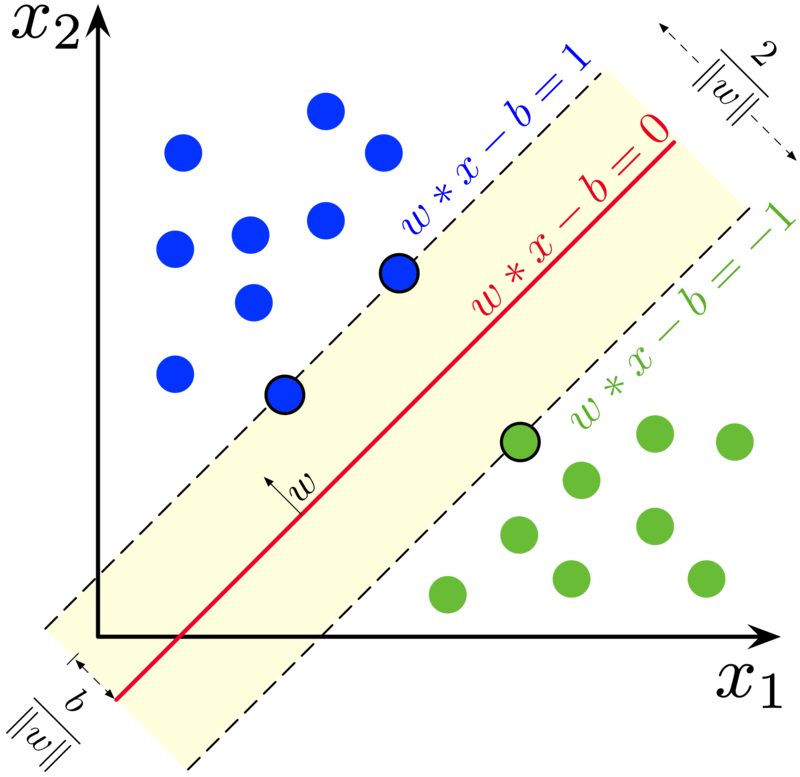
\includegraphics[scale=1.8]{svm-1.png}
\captionof{figure}{Hyperplane construction in SVM}
\label{fig:svm-1}
\end{center}

\noindent SVMs are supervised learning models used for regression and classification tasks. For classification, two hyperplanes are constructed, separating linearly separable data classes. The hyperplane at the midway of these two planes is the maximum hyperplane which acts as a classification boundary (Fig. \ref{fig:svm-1}).

\vskip 0.2in
\begin{center}
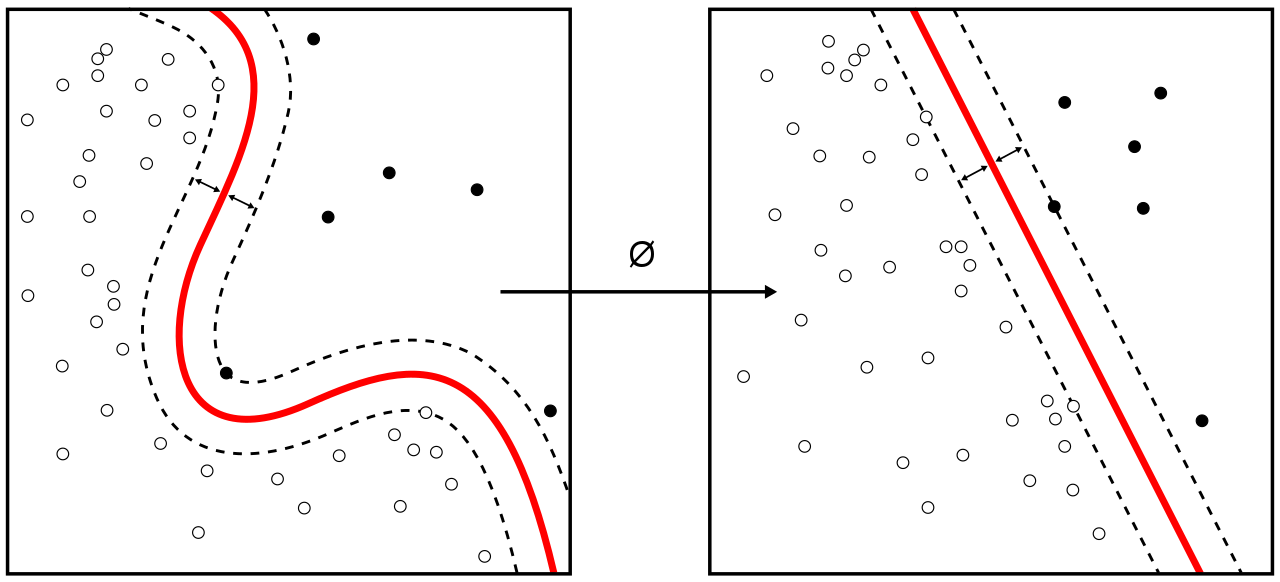
\includegraphics[scale=0.2]{svm-2.png}
\captionof{figure}{Kernel mapping to linear boundaries}
\label{fig:svm-2}
\end{center}
\noindent 
For non-linear data, a kernel is used, which is a function mapping the data into higher dimensional linear feature space (Fig. \ref{fig:svm-2})


\vskip 0.2in
\subsubsection{K-Nearest Neighbours (KNN)}
\begin{center}
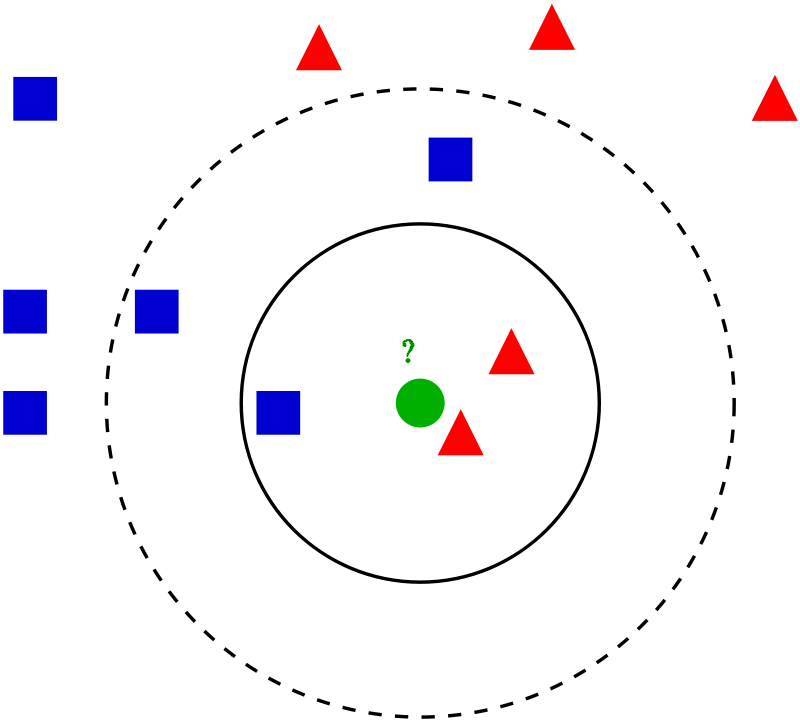
\includegraphics[scale=0.3]{knn.png}
\captionof{figure}{Example of KNN}
\label{fig:knn}
\end{center}
\noindent KNN is a supervised algorithm for supervised classification and regression tasks. KNN works by finding the \(K\) closest data points to a given query point. The output is the most frequent label for classification and the mean of the label for regression tasks. The value of \(K\) is user-defined as a hyperparameter, and the distance metric is euclidean or hamming distance depending on the context of the dataset.

\vskip 0.2in
\subsubsection{Bayesian Network (BN)}
\noindent A BN is a Directed Acyclic Graph (DAG) used to represent the probabilistic dependencies of a collection of random variables. Each node of the BN represents a random variable, and each edge between the nodes represents the conditional probability between the nodes, which is derived from the Bayes theorem:
\begin{equation}
    P(A|B) = \frac{P(B|A)P(A)}{P(B)}
\end{equation}
As an example, consider the BN in (Fig. \ref{fig:bn}), modelling the conditions when the grass can be wet. If it rains or the sprinklers are active, there is a higher probability of grass being wet. Moreover, if it is raining, the probability of the sprinkler being kept active is lesser.
\begin{center}
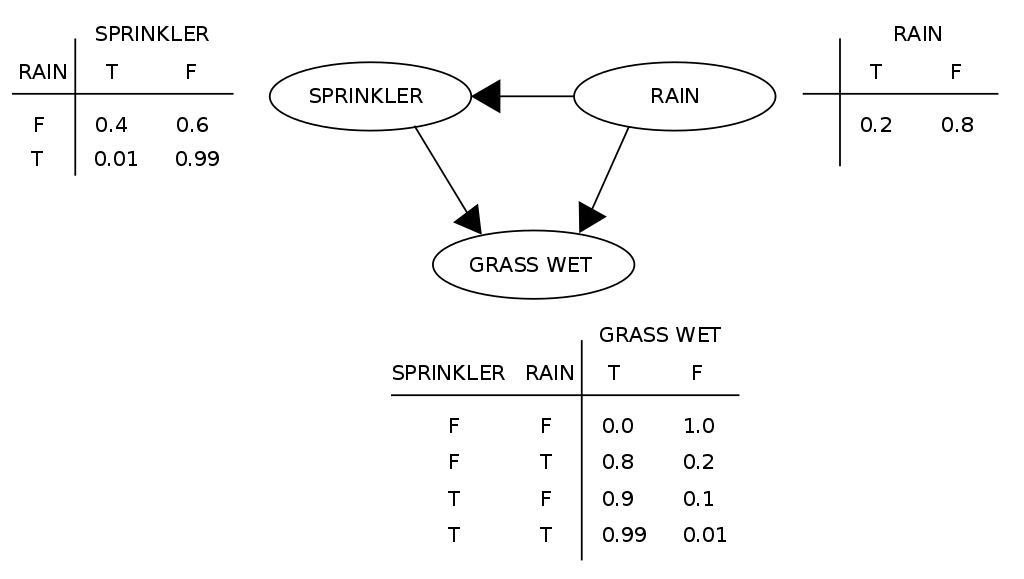
\includegraphics[scale=0.3]{bn.png}
\captionof{figure}{Example of BN}
\label{fig:bn}
\end{center}

\vskip 0.2in
\subsubsection{Linear Discriminant Analysis (LDA)}
\begin{center}
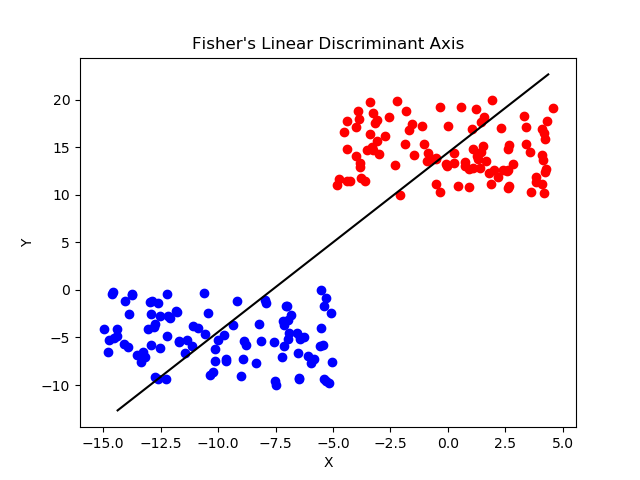
\includegraphics[scale=0.8]{lda.png}
\captionof{figure}{Fisher's LDA Visualization}
\label{fig:lda}
\end{center}

\noindent LDA is used for dimensionality reduction, especially for supervised classification tasks to separate two or more classes spatially. LDA takes a component of the data points on a single axis tuned to maximize the distance between two classes and minimize the variation within members of a single class.

\vskip 0.2in
\subsubsection{Artificial Neural Networks (ANN)}

\noindent ANNs are machine learning models mimicking biological neural networks. An ANN consists of neuron layers where each layer contains an array of artificial neurons. These neurons are essentially mathematical functions that take input values from previous layers and are tunable using a set of weights and biases. ANNs are used for supervised, unsupervised as well as reinforcement learning tasks.

\begin{center}
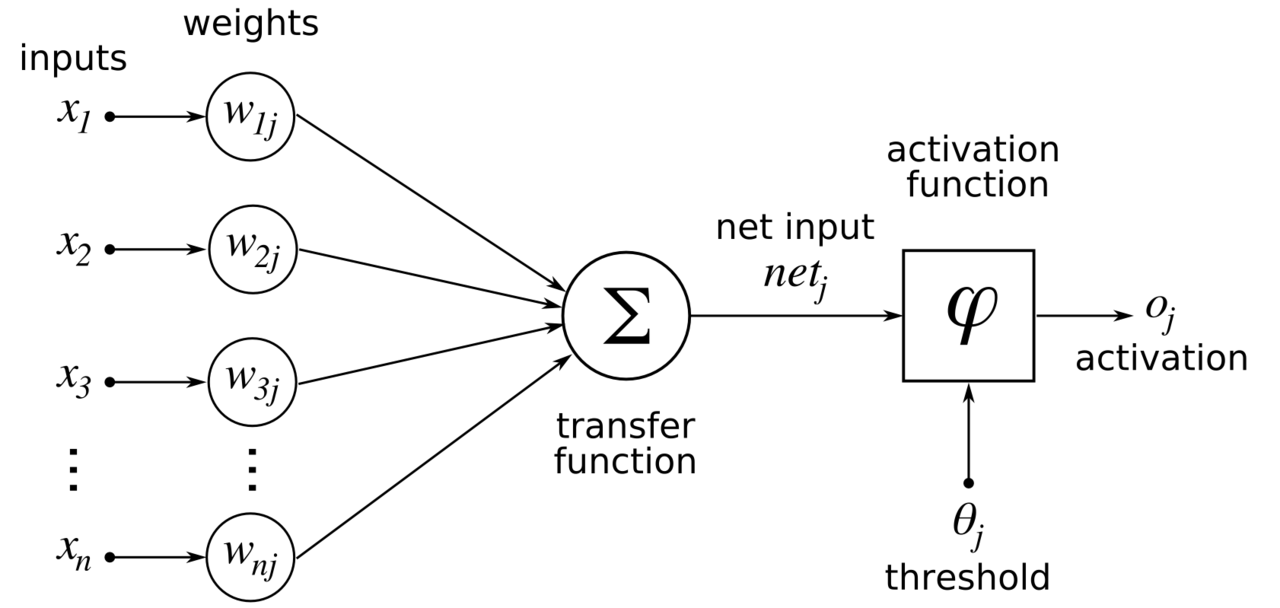
\includegraphics[scale=0.38]{ann.png}
\captionof{figure}{Single neuron in an ANN}
\label{fig:ann}
\end{center}

\vskip 0.2in
\noindent\textbf{Multilayer Perceptron (MLP)} \\
\noindent MLPs are a class of feedforward ANNs where the connections between layers of neurons are unidirectional and acyclic. Each neuron is an activation function like hyperbolic tan, logistic function and rectifier function.
\begin{equation}
    y(v_i) = \tanh(v_i)
\end{equation}
\begin{equation}
    y(v_i) = \frac{1}{1 + e^{v_i}}
\end{equation}
\begin{equation}
    y(v_i) = \max(0, v_i)
\end{equation}

\vskip 0.2in
\subsection{Overview Banking and Risk Management Terminologies}
\subsubsection{Risk}
\noindent Risk in finance is defined as uncertainty or volatility of unexpected outcomes, representing the value of assets, equity, or earnings. This includes both positive as well as negative outcomes. A higher return is associated with a more significant variability of outcomes \cite{jorion2000value}. Risk is broadly classified into Credit Risk, Market Risk, Liquidity Risk and Operational Risk.
\vskip 0.2in
\subsubsection{Credit Risk}
\noindent Credit risk is the risk of defaulting on bank loans or failing to comply with the debt obligations of a borrower \cite{kanchu2013risk}. Credit risk also refers to the decline of a borrower's credit quality, which does not directly indicate default but involves a higher probability of default. The book value does not change when the borrower's credit quality diminishes, but its economic value is lower because the probability of default increases \cite{bessis2011risk}.

\vskip 0.2in
\subsubsection{Market Risk}
\noindent Market risk is the risk of the movement of market prices. Prices of market parameters that fluctuate randomly include equity indexes, commodity prices, interest rates and foreign exchange rates \cite{bessis2011risk}.

\vskip 0.2in
\noindent\textbf{Time Series Forecasting} \\
\noindent Time Series Forecasting is used to predict the market price movement. It involves conceptualizing statistical and machine learning models to predict future values based on previously observed values.

\vskip 0.2in
\noindent\textbf{Innovation} \\
\noindent Innovation is the difference between a forecast made by a statistical algorithm and the actual value for a time-varying function.

\vskip 0.2in
\noindent\textbf{Heteroscedasticity} \\
\noindent Heteroscedasticity is the variance or volatility observed in a time-varying random function.

\vskip 0.2in
\subsubsection{Liquidity Risk}
\noindent Liquidity is the ease with which a financial instrument can be exchanged for money without losing value. High liquidity indicates a high supply and demand for an asset, which means there will always be buyers and sellers. Liquidity risk is the uncertainty linked with the outcome and possible losses of such an asset transaction into funds \cite{tavana2018artificial}.

\vskip 0.2in
\noindent\textbf{Measuring Liquidity} \\
\noindent Liquidity is measured using ratios like Liquidity Coverage Ratio (LCR) and Net Stable Funding Ratio (NSFR). LCR measures the number of liquid assets a bank has to cover for any short term liquid fund requirements. NSFR, on the other hand, measure a bank's long term resilience to liquidity risks. Basel Norms require that both the ratios must be maintained above 100\% by banks.

\begin{equation}
    LCR = \frac{\text{stock of high quality liquid assets}}{\text{total net cash} - \text{flow over the next 30 days}}
\end{equation}

\begin{equation}
    NSFR = \frac{\text{available amount of stable funding}}{\text{required amount of stable funding}}
\end{equation}

\vskip 0.2in
\subsubsection{Operational Risk}
\noindent Operational Risk is the risk associated with failures in internal procedures, external events, and infrastructure. Fraud detection, cyber security attacks, suspicious transaction detection, money laundering all come under the radar of operational risk \cite{bessis2011risk}.

\vskip 0.2in
\noindent\textbf{Money Laundering} \\
\noindent Money Laundering converts substantial amounts of funds earned from crimes and terrorism into origination from a legitimate source. This is accomplished by routing transactions through numerous layers of legal transactions to hide the natural source of income.

\vskip 0.2in
\subsection{Summary}
In conclusion, this chapter briefly introduces various concepts and terminologies that would be a prerequisite for Chapter 3 and Chapter 4. Machine learning algorithms are used to solve a vast array of economics, banking, and risk management problems.

\newpage
\section{\centering Literature Review}
\vskip 0.25in
This chapter discusses various contributions of researchers and scholars for Risk Management in Banking using Machine Learning Models.

\vskip 0.2in
\subsection{Credit Risk}
Credit Risk analysis is the fundamental problem of the lending economy, with initial efforts dating back to the 20th century. The financial recessions of the 21st century and the ever-increasing complexity of regulatory constraints have led to increased academic and business efforts towards the problem. From a Machine Learning perspective, evaluating credit risk involves binary classification: Determining if a potential customer is credit-worthy from their financial history.

\vskip 0.2in
\subsubsection{Traditional Machine Learning Algorithms for Credit Scoring}
\noindent A family of statistical frameworks have been adopted since the early 1900s for credit scoring potential borrowers. Among the traditional classifiers, SVMs have yielded significantly better results.
\\
\\
\noindent Bellotti et al. tested the performance of SVMs for credit score classification and contrasted the results with traditional approaches \cite{bellotti2009support}. The paper compares the performance of different algorithms like LR, SVM, LDA and KNN. The work concluded with LDA and SVM reporting the highest AUC scores for the ROC curves when trained on a dataset of about 25,000 over three months of 2004 for credit card based lending \cite{bellotti2009support}. However, SVMs are very sensitive to the outliers of the datasets. Wang et al. introduced a fuzzy SVM algorithm for the classification task to reduce this sensitivity and increase the generalization of the data \cite{wang2005new}.

\vskip 0.2in
\subsubsection{Neural Networks for Credit Scoring}
\noindent Early works in the area primarily included the use of SVM based algorithms. However, with larger datasets, training becomes computationally expensive \cite{harris2015credit}. ANNs have been widely researched for credit scoring \cite{li2002neural, hu2006ann}. Several Ensemble methods have been employed to improve the accuracy of the ANN models \cite{tsai2008using}.
\\
\\
Angelini et al. used ANNs to determine credit risk among small businesses as credit borrowers \cite{angelini2008neural}. The work proposes a real-world dataset of Italian businesses and provides a comprehensive network performance analysis for various neuron configurations.
\\
\\
Tsai et al. employed a single MLP classifier as a benchmark for prediction accuracy and compared the performance with multiple classifiers in the ensembled form \cite{tsai2008using}. The paper also reports the variation in accuracy by modifying training configuration parameters like the number of epochs, network architecture, and the number of classifiers for ensembling. The analysis is performed on the publicly available Australian, German and Japanese credit datasets.


\vskip 0.2in
\subsection{Market Risk}
\noindent Market risk deals with the volatility of indices. Value at Risk (VAR) estimates the worst loss that will not exceed in a particular time frame. It captures the combined effect of underlying volatility and exposure to financial risks. Volatility estimation is a part of the time series forecasting domain. ANNs excel at these learning problems compared to traditional methods. A commonly used forecasting framework for time series is the Generalized Autoregressive Conditional Heteroskedasticity (GARCH) model \cite{bollerslev1986generalized}. It is derived from the Autoregressive Conditional Heteroscedasticity (ARCH) model, which predicts the volatility of innovation or error term as a function of previous error terms.
\\
\\
The volatility at time \(t\) is given as a function of prior error terms as:

\begin{equation}
    \sigma_t^2 = \alpha_0 + \sum_{i = 1}^{n} \alpha_i \epsilon_{t - i}^2
\end{equation}

\noindent GARCH model also considers the volatility of prior time to predict the current volatility:

\begin{equation}
    \sigma_t^2 = \ \omega + \sum_{i = 1}^{n} \alpha_i \epsilon_{t - i}^2 + \sum_{i = 1}^{p} \beta_i \sigma_{t - i}^2
\end{equation}

\noindent Zhang et al. proposed a model to calculate the VAR (volatility) in an index from the GARCH model using ANNs \cite{zhang2017calculating}. The paper also presents a comparative analysis with other models like just GARCH and SVM to predict volatility.

\vskip 0.2in
\subsection{Liquidity Risk}
\noindent Liquidity risk is the risk of not being equipped to raise capital when required. Trading of financial instruments and assets enable the raising of capital to banking institutions. Such funding is known as funding liquidity. When it is difficult to borrow or raise money, liquidity risk comes into play. For example, banks faced heavy losses in the 2008 crisis when assets were trading at heavily discounted rates due to the crash and the banks urgently needed funds to keep their businesses running.
\\
\\
\noindent Machine learning can solve several liquidity risk factors. ANNs can be used to estimate a risk measure. Approximation of general risk trends and discovery of principal risk determinants can be made using ANNs. BN can be used to predict the probability of a liquidity risk event happening.  By using distributive estimation, the ANN and BN implementations could identify the most critical liquidity risk factors.
\\
\\
\noindent Tavana et al. used a combination of ANN and BN to determine liquidity risk (LCR and NSFR) from a real-world dataset of a U.S. bank focusing mainly on loans for eight consecutive years. The ANN was used to approximate the general trend of liquidity risk and find the influential factors. Further, the BN was used to find the most influential factor from the data filtered by the ANN \cite{tavana2018artificial}.

\vskip 0.2in
\subsection{Operational Risk}
\noindent Operational Risk arises due to malfunctions in internal and external processes. Machine Learning is used in an operational context to detect such malfunctions. Fraud detection is a significant area of focus of operational risk management.
\\
\\
\noindent Money laundering is the malpractice of hiding illegal sources of income by layering lawful transactions on such sources. This is done by routing money through many complicated but legitimate transactions to conceal the actual source. These funds are further used to support criminal, war and terrorist activities.
\\
\\
\noindent Sudjianto et al. employed clustering algorithms to segment customers based on transaction activity \cite{sudjianto2010statistical}. The work combines clustering and profiling to perform unsupervised peer group analysis (PGA) \cite{bolton2001peer}. These segments are used for analyzing if the group of customers were involved in money laundering. Another challenge in identifying fraud is to flag suspicious transactions first and then perform an anti-money laundering investigation. The paper also presents classifiers like LR, SVM, CART, C4.5, C5.0 and RF for determining illegal transactions.
\\
\\
\noindent Villalobos et al. has done comparable work on money laundering detection using ANN, SVM and C5.0 based classifiers \cite{villalobos2017statistical}. The experiments were performed on a Latin American financial institution dataset, and decision tree-based classifiers excelled at the task compared to other models. 

\begin{table}[H]
\captionof{table}{Literature Survey Summary}
\label{table2}
\vskip 0.1in
\bgroup
\def\arraystretch{1.5}
\begin{tabular}{ | p{1.9cm} | p{1.6cm}| p{2.1cm} | p{1.4cm}| p{2.3cm}| p{1.9cm}| p{2.2cm}| }
\hline
\textbf{Task} & \textbf{Author}  & \textbf{Title}  & \textbf{Model} & \textbf{Performance Measure}  & \textbf{Dataset}  & \textbf{Features} \\
  \hline
Credit Risk &
Bellotti et al. \cite{bellotti2009support} &
Support vector machines for credit scoring and discovery of significant features &
SVM, LR, KNN, LDA &
AUC &
Credit card history of 25,000 customers over a three month period &
34 features taken from each customer’s original application and features extracted from a credit reference agency
\\
 \hline
 Credit Risk &
Tsai et al. \cite{tsai2008using} &
Using neural network ensembles for bankruptcy prediction and credit scoring &
MLP, Ensembled MLP &
Accuracy, Type I and Type II errors &
Australian, German and Japanese credit datasets &
20 attributes including age, gender, amount and duration of credit and job status
\\
\hline

Credit Risk &
Wang et al. \cite{wang2005new} &
A new fuzzy support vector machine to evaluate credit risk &
Fuzzy SVM &
Type I and Type II and overall accuracy &
FAME, Japanese credit dataset &
12 features for FAME, 15 for the Japanese credit dataset 
\\
\hline


\end{tabular}
\egroup
\end{table}
\newpage
\begin{table}[H]
\bgroup
\def\arraystretch{1.5}
\begin{tabular}{ | p{1.9cm} | p{1.6cm}| p{2.1cm} | p{1.4cm}| p{2.3cm}| p{1.9cm}| p{2.2cm}| }
\hline
\textbf{Task} & \textbf{Author}  & \textbf{Title}  & \textbf{Model} & \textbf{Performance Measure}  & \textbf{Dataset}  & \textbf{Features} \\
 \hline

Credit Risk &
Angelini et al. \cite{angelini2008neural} &
A neural network approach for credit risk evaluation &
ANN &
Error &
Italian small business dataset &
15 features derived from the balance sheet of the small businesses
\\
\hline

Market Risk &
Zhang et al. \cite{zhang2017calculating} &
Calculating Value-at-Risk for high-dimensional time series using a nonlinear random mapping model &
GARCH, ANN &
p-value &
China Securities Index 300 from April 8, 2005, to May 28, 2015 &
Daily closing price
\\
\hline

Liquidity Risk &
Tavana et al. \cite{tavana2018artificial} &
An Artificial Neural Network and Bayesian Network model for liquidity risk assessment in banking &
ANN, BN &
MSE &
Dataset of a U.S. bank focusing mainly on loans from 2004 to 2011 &
Liquid assets of bank, Current liabilities, short and long term deposits, total assets 
\\
\hline

Operational Risk &
Sudjianto et al. \cite{sudjianto2010statistical} &
Statistical methods for fighting financial crimes &
LR, SVM, DT, RF, PGA &
Error &
AML Dataset &
Account number, transaction amount, date, description
\\
\hline


Operational Risk &
Villalobos et al. \cite{villalobos2017statistical} &
A statistical and machine learning model to detect money laundering: an application &
ANN, SVM, C5.0 &
Accuracy, AUC &
Latin American Financial Institution data &
Customer nationality, type of entity, source of assets, reputation risk score, owners risk rating 
\\
\hline


\end{tabular}
\egroup
\end{table}

\vskip 0.2in
\subsection{Summary}
This chapter presents a comprehensive survey of various types of machine learning and statistical techniques used to solve risk management problems in finance. An interesting observation is that certain types of machine learning models perform better at specific risk management tasks. This is reflected by the number of academic works published for such algorithm-problem pairs. For example, SVMs have been extensively used for credit scoring tasks while tree-based classifiers excel at fraud detection tasks. Nevertheless, ANN seems to have found applications in all types of problems explored and produced state of the art results in many banking problems.


\newpage
\section{\centering Case Study in Credit Risk}
\vskip 0.25in
This chapter reports and analyzes the performance of various machine learning models on the credit risk classification task. The publicly available German Credit Score dataset is used to train the following classifiers: LR, LDA, KNN, CART, C5.0, NB, RF, SVM and ANN.

\vskip 0.2in
\subsection{German Credit Dataset}
This dataset classifies customers as having good or bad credit potential by a set of attributes. It contains 1000 instances of data points and 20 attributes for each data point. These features capture information like:
\begin{itemize}
  \item Status of bank accounts
  \item Purpose of loan
  \item Amount and duration of loan
  \item Age, gender and employment of the customer
  \item Credit history
  \item Mode of repayment
\end{itemize}

\vskip 0.2in
\subsection{Exploratory Data Analysis (EDA)}
\subsubsection{Distribution of Good and Bad Credit}
\noindent The dataset contains 700 examples for the "Good Credit" rating and 300 examples for the "Bad credit" rating. This creates an imbalance in the dataset, which can degrade classification quality. Random oversampling is done to rebalance the dataset before feeding it to the models. \cite{japkowicz2002class}


\begin{center}
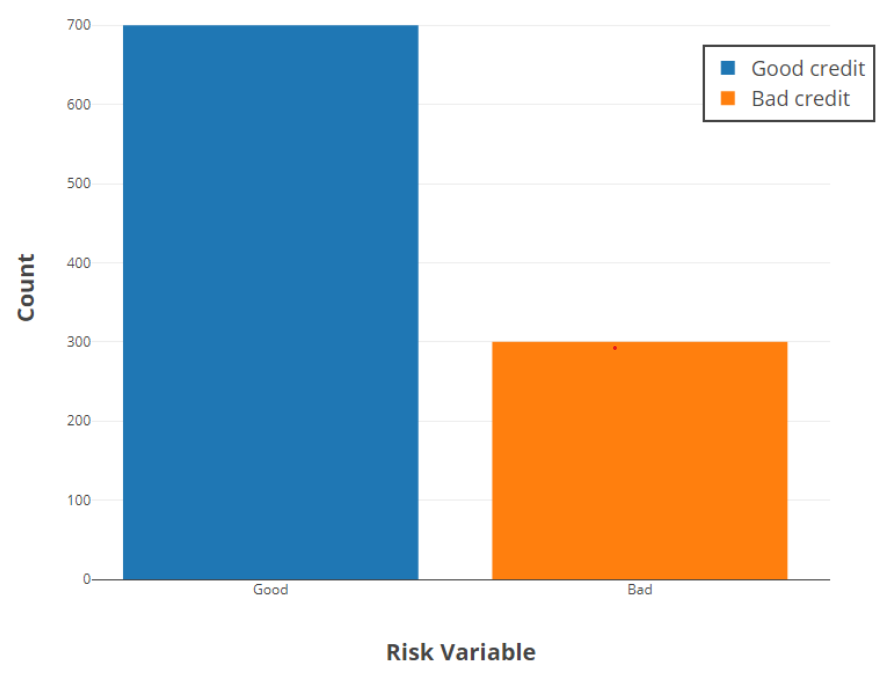
\includegraphics[scale=0.6]{dist-1.png}
\captionof{figure}{Distribution of good and bad credit}
\label{fig:dist1}
\end{center}

\subsubsection{Age Distribution}
\noindent (Fig. \ref{fig:dist2}) shows the distribution of loans with age. The distribution is shown based on the classification target as well as a combined graph. An interesting observation is that bad credit loans taper off quickly as age increases compared to the good credit loans, thus indicating that the younger audience may have a significant contribution in non-payment of loans.

\begin{center}
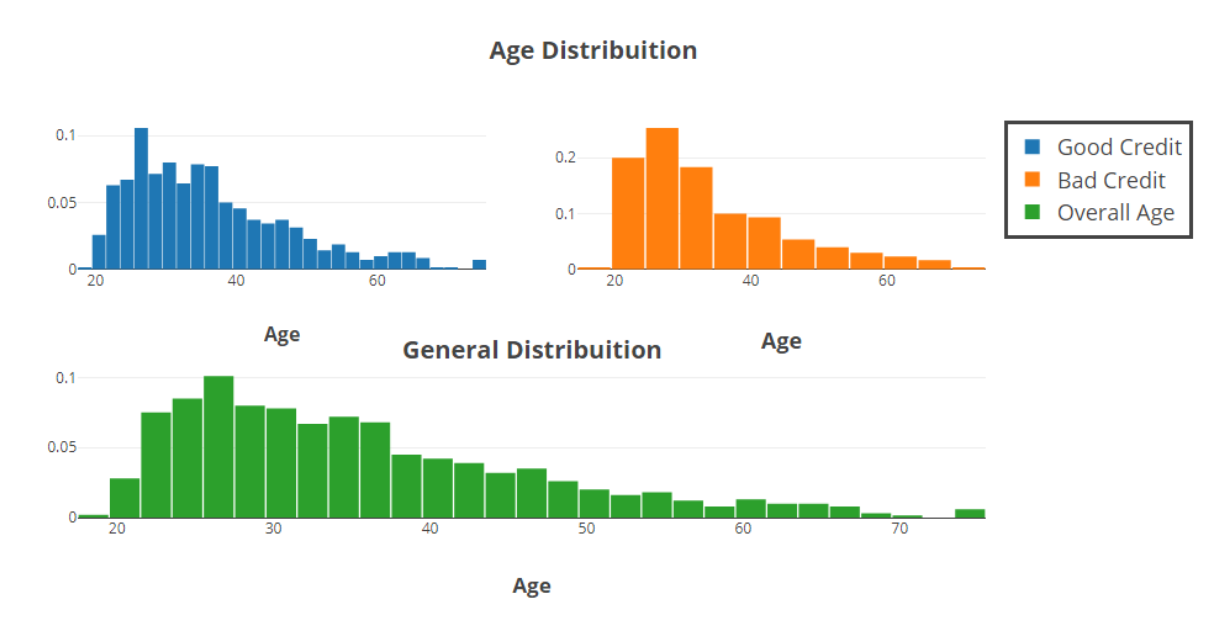
\includegraphics[scale=0.4]{dist-2.png}
\captionof{figure}{Distribution of credit based on age}
\label{fig:dist2}
\end{center}

\subsubsection{House Type Distribution}

\begin{center}
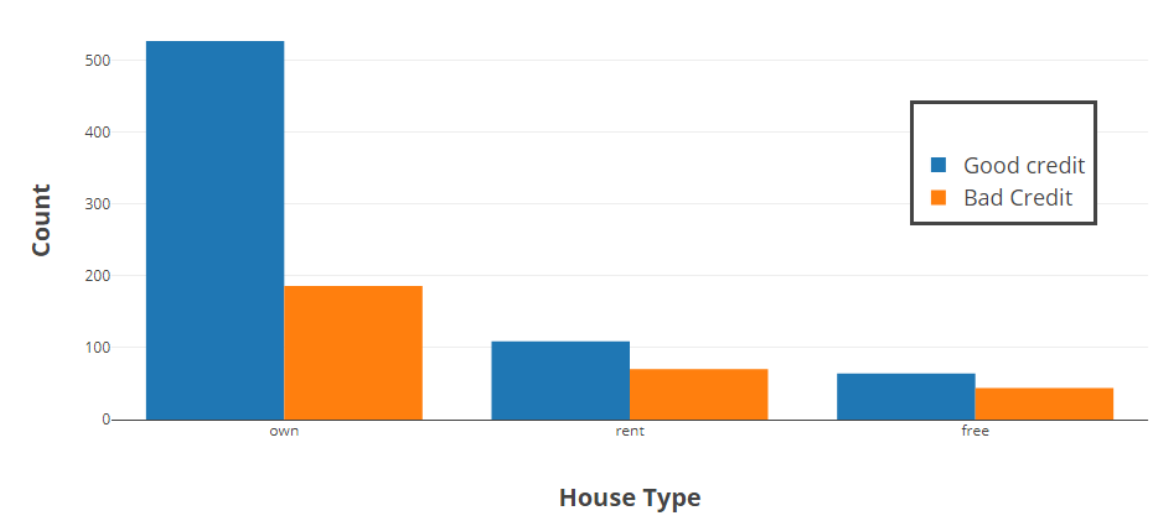
\includegraphics[scale=0.4]{dist-3.png}
\captionof{figure}{Distribution of credit based on purpose}
\label{fig:dist3}
\end{center}

\noindent People who own their own house are more likely to pay off their loans. On the other hand, there is almost a 40\% chance that the loan will have defaulted for the other two classes.

\subsubsection{Loan Purpose Distribution}

\begin{center}
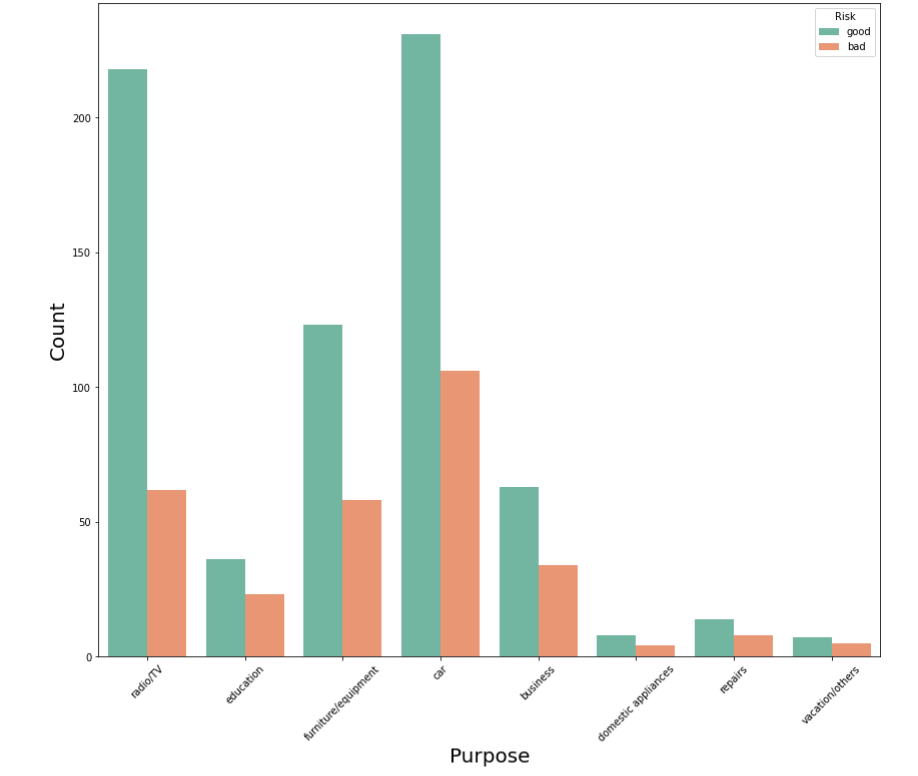
\includegraphics[scale=0.6]{dist-4.png}
\captionof{figure}{Distribution of credit based on purpose}
\label{fig:dist4}
\end{center}

\noindent Loans are mainly taken to buy a car or TV. Credit taken to buy TV/Radio has the least risk of default. Education and Vacation loans carry a higher credit risk, which parallels with banks charging a higher rate of interest for education loans to account for the risk of default.


\subsection{Results}
Before training, the minority class was oversampled to meet the size of the majority class. The data was split into a 1:4 ratio with the larger portion used to train the models, and the smaller portion is used for evaluation. Five trials were carried out for each classifier, and their average performance metrics are reported in Table \ref{table:4}.

\vskip 0.2in
\begin{table}[h!]
\caption{Performance of classifiers on German Credit Dataset}
\label{table:4}
\begin{tabularx}{1.0\textwidth} { 
  | >{\raggedright\arraybackslash}X 
  | >{\raggedright\arraybackslash}X 
  | >{\raggedright\arraybackslash}X 
  | >{\raggedright\arraybackslash}X|}
 \hline
 \textbf {Model} & \textbf{Accuracy} & \textbf{F1 Score} & \textbf{AUC} \\
 \hline
 \textbf{LR} & 0.7285 & 0.7300 & 0.7292 \\
\hline
\textbf{LDA} & 0.7188 & 0.7196 & 0.7196  \\
\hline
\textbf{KNN} & 0.7240 & 0.7406 & 0.7226 \\
\hline
\textbf{CART} & 0.8417 & 0.8529 & 0.8387 \\
\hline
\textbf{C5.0} & 0.8428 & 0.8557 & 0.8408 \\
\hline
\textbf{RF} & 0.8754 & 0.8820 & 0.8746 \\
\hline
\textbf{NB} & 0.7023 & 0.7112 & 0.7019 \\
\hline
\textbf{SVM} & 0.7955 & 0.8054 & 0.7959 \\
\hline
\textbf{ANN} & 0.7509 & 0.7586 & 0.7505 \\
\hline
\end{tabularx}
\end{table}

\noindent For each model, Receiver Operating Characteristics (ROC) curves are plotted in (Fig. \ref{fig:roc}).

\begin{center}
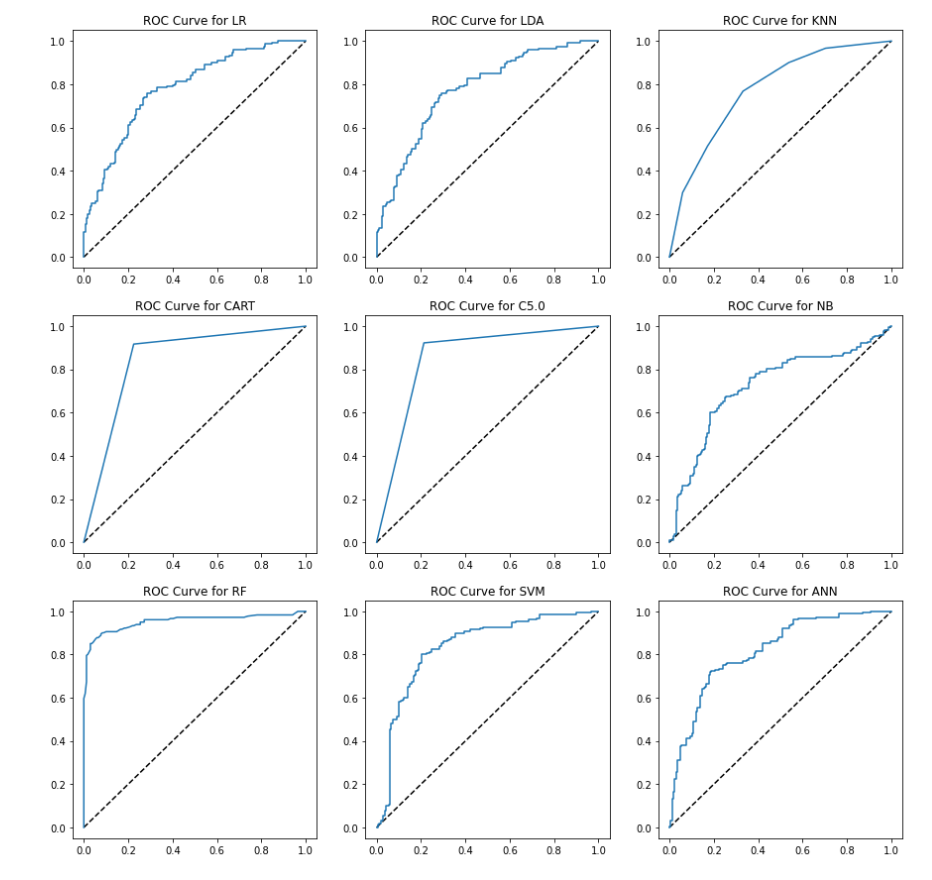
\includegraphics[scale=0.7]{roc.png}
\captionof{figure}{ROC for classifiers}
\label{fig:roc}
\end{center}

\noindent In summary, both the tree-based algorithms (CART and C5.0) performed better than other models with an F1 score greater than 0.8. When ensemble learning is used in the RF classifier, the best results are achieved with a 0.88 F1 score, which is reflected in the ROC curve. SVM and ANN are the next best classifiers for the learning task respectively.

\newpage
\section{\centering Conclusion}
\vskip 0.25in
Throughout all modern human history, banking has been an essential factor in fueling innovation and betterment of the society. With the coming of the information age, increased competition and modern banking facilities available to the commoner, risk management plays a vital role in building a sustainable and compliant banking business. Banks generate several terabytes of data that state-of-the-art machine learning models can leverage to make data-driven decisions. In this report, various machine learning applications for risk management in banking are presented. This work does a comprehensive survey of academic research for different risk management areas viz. credit risk, operational risk, market risk and liquidity risk. A case study is also presented comparing the performance of various classifiers like ANNs, DTs, SVM and others on a single dataset for credit scoring tasks.


\newpage
% \textbf{
% {\fontsize{18pt}{18pt}\selectfont References} 
% }\\
% \addcontentsline{toc}{chapter}{References}
% \printbibliography
\phantomsection
\addcontentsline{toc}{section}{References}
\printbibliography[heading={References}, title=References]
\newpage
\phantomsection
\section*{\centering Acknowledgment}
\addcontentsline{toc}{section}{Acknowledgment}
\vskip 0.2in
\raggedright I would like to express my deep gratitude and indebtedness to my project guide, Dr Rupa G. Mehta, Associate Professor, Computer Engineering Department, SVNIT Surat, for her valuable guidance, constructive feedback and co-operation with a kind and encouraging attitude for the successful completion of this work. I would also like to thank Dr Mukesh A. Zaveri, Head of Department, Computer Engineering Department. I am also thankful to the Computer Engineering Department faculties for direct or indirect support to complete this seminar.
\end{document}
